\documentclass{article}

\usepackage{postprocess/context/arxiv}

\usepackage[utf8]{inputenc} % allow utf-8 input
\usepackage[T1]{fontenc}    % use 8-bit T1 fonts
\usepackage{hyperref}       % hyperlinks
\usepackage{url}            % simple URL typesetting
\usepackage{booktabs}       % professional-quality tables
\usepackage{amsfonts}       % blackboard math symbols
\usepackage{nicefrac}       % compact symbols for 1/2, etc.
\usepackage{microtype}      % microtypography
\usepackage{lipsum}		% Can be removed after putting your text content
\usepackage{graphicx}
\usepackage{natbib}
\usepackage{doi}
\usepackage{float}
\usepackage{subcaption}

\title{Causal Discovery Report on Dwd}

\author{ \href{https://orcid.org/0000-0000-0000-0000}{
\includegraphics[scale=0.06]{postprocess/context/orcid.pdf}\hspace{1mm}Causal Copilot}}

\renewcommand{\headeright}{Technical Report}
\renewcommand{\undertitle}{Technical Report}

\hypersetup{
pdftitle={Causal Discovery Report on Dwd},
pdfauthor={Causal Copilot},
pdfkeywords={Causal Discovery, Large Language Model, PC, Dwd},
}

\begin{document}
\maketitle

\begin{abstract}
This report investigates the causal relationships among environmental and meteorological variables, namely altitude, temperature, precipitation, longitude, and sunshine hours, utilizing a data-driven approach to enhance our understanding of climate dynamics. The methodology involves a comprehensive causal discovery process aided by a large language model (LLM) to select suitable algorithms—PC, GES, and NOTEARS—based on statistical characteristics of the data. Preprocessing steps were performed to clean the data and manage missing values, followed by the selection of specific hyperparameters for optimal causal inference. The results indicate complex interdependencies, revealing that altitude significantly impacts both temperature and precipitation, while longitude plays a critical role in influencing temperature and sunshine hours. The findings contribute to the field by providing a refined causal graph that elucidates the interactions among these climatic factors, supported by both statistical evidence and expert knowledge, thus laying the groundwork for future investigations into climate-related phenomena.
\end{abstract}

\keywords{Causal Discovery, Large Language Model, PC, Dwd}

\raggedbottom
\section{Introduction}
In this report, we aim to explore the causal relationships among a set of environmental and meteorological variables, namely altitude, temperature, precipitation, longitude, and sunshine hours. Each of these variables plays a critical role in understanding climate dynamics and ecological interactions. For instance, altitude is known to influence both temperature and precipitation patterns, while temperature can significantly affect evaporation rates and thus precipitation outcomes. Additionally, the geographical positioning denoted by longitude may contribute to local climate variations, impacting temperature distributions. Sunshine hours further modulate temperature and precipitation, suggesting potential interconnectedness among these factors. Utilizing statistical methods for causal discovery, we will investigate the underlying mechanisms that govern these relationships, drawing on insights from climatology, ecology, and agricultural science to enhance our understanding of how these variables interact and influence one another.

\section{Background Knowledge}
\subsection{Detailed Explanation about the Variables}
\begin{itemize}
\item \textbf{Altitude}: This variable represents the height of a location above sea level, usually measured in meters. Altitude can have a significant effect on various environmental factors, including temperature, precipitation, and biodiversity.
\item \textbf{Temperature}: This variable indicates the degree of heat present in the atmosphere, typically measured in degrees Celsius (°C). Temperature is a crucial factor in determining weather patterns and ecological conditions.
\item \textbf{Precipitation}: This variable refers to the amount of water, in the form of rain, snow, sleet, or hail, that falls to the earth's surface over a defined period. It is measured in millimeters (mm). Precipitation is vital for understanding water availability in ecosystems and agricultural settings.
\item \textbf{Longitude}: This variable specifies the east-west position of a point on the Earth's surface, measured in degrees. Longitude is important for geographical orientation and can be used in analyses that account for geographical variations in climate and weather patterns.
\item \textbf{Sunshine hours}: This variable measures the amount of time (usually in hours) that sunlight is received at a specific location during a given period. Sunshine hours influence temperature and can also affect vegetation and agricultural yields.
\end{itemize}

\subsection{Possible Causal Relations among these Variables}
\begin{minipage}[t]{0.7\linewidth}
    \begin{itemize}
    \item \textbf{Altitude $\rightarrow$ Temperature}: Typically, as altitude increases, the temperature tends to decrease due to the thinning atmosphere at higher elevations, resulting in a cooler climate.
    \item \textbf{Temperature $\rightarrow$ Precipitation}: Higher temperatures can lead to increased evaporation rates, causing more moisture in the atmosphere. This can result in increased precipitation as warmer air can hold more water vapor, leading to clouds and eventual rainfall or snowfall.
    \item \textbf{Altitude $\rightarrow$ Precipitation}: Higher altitudes can enhance orographic lifting, where moist air is forced to rise over mountains, cooling and condensing to produce greater precipitation in these elevated areas.
    \item \textbf{Longitude $\rightarrow$ Temperature}: The longitudinal position can influence climate due to the different thermal properties of land and water bodies, as well as variations in predictable weather patterns, which alter temperature profiles across different regions.
    \item \textbf{Sunshine Hours $\rightarrow$ Temperature}: An increase in sunshine hours generally leads to higher temperatures, as more solar radiation contributes to heating the earth's surface, influencing local temperature measurements throughout various times of the day and year.
    \item \textbf{Sunshine Hours $\rightarrow$ Precipitation}: Areas characterized by higher sunshine hours often have lower precipitation levels, especially in arid or semi-arid climates, while regions with fewer sunshine hours may experience higher instances of precipitation due to increased cloud cover and moisture retention.
    \item \textbf{Temperature $\rightarrow$ Sunshine Hours}: Higher temperatures can lead to fewer clouds and clearer skies, resulting in increased sunshine hours in a location, thereby reinforcing a feedback loop where temperature and sunshine influence each other.
    \item \textbf{Longitude $\rightarrow$ Precipitation}: Longitude can also determine precipitation patterns as it affects the proximity to oceanic influences, which provide moisture necessary for precipitation, indicating a complex interaction with regional climatic changes.
\end{itemize}
\vfill
\end{minipage}
\hspace{0.05\textwidth}
\begin{minipage}[t]{0.3\linewidth}
    \begin{figure}[H]
        \centering
        \vspace{-0.5cm}
        \resizebox{\linewidth}{!}{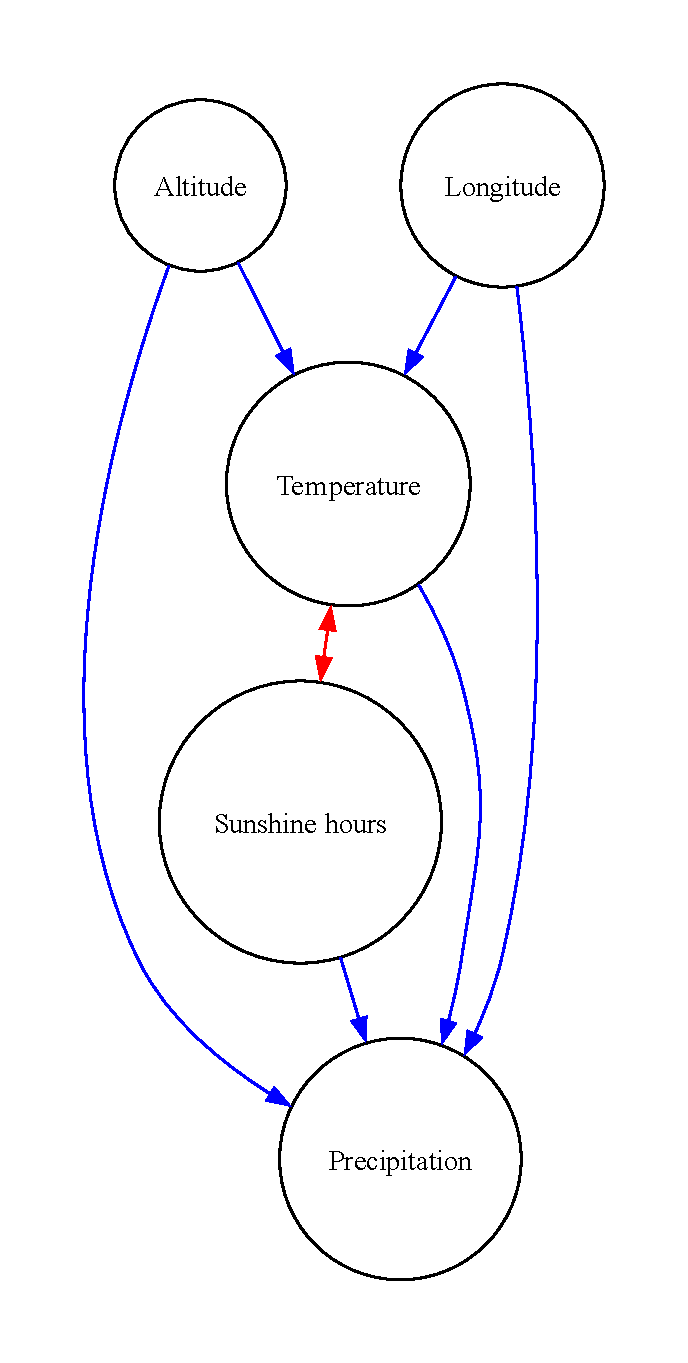
\includegraphics[height=0.4\textheight]{dataset/DWD/output_graph/potential_relation.pdf}}
        \caption{\label{fig:relation}Possible Causal Relation Graph}
    \end{figure}
\end{minipage}

\section{Dataset Descriptions and EDA}
The following is a preview of our original dataset.

\begin{table}[H]
    \centering
    \caption{Dataset Preview}
    \begin{tabular}{rrrrr}
\toprule
 Altitude &  Temperature &  Precipitation &  Longitude &  Sunshine hours \\
\midrule
    205.0 &          9.7 &          828.3 &       6.08 &          1552.0 \\
     46.0 &          8.2 &          791.5 &      10.20 &          1443.3 \\
    794.0 &          6.4 &         1057.8 &       9.00 &          1096.5 \\
    325.0 &          8.1 &          803.0 &      13.08 &          1571.7 \\
    500.0 &          6.2 &         1252.2 &      10.43 &          1368.0 \\
\bottomrule
\end{tabular}
\end{table}

\subsection{Data Properties}
We employ several statistical methods to identify data properties.

The shape of the data, data types, and missing values are assessed directly from the dataframe. Linearity is evaluated using Ramsey’s RESET test, followed by the Benjamini \& Yekutieli procedure for multiple test correction. Gaussian noise is assessed through the Shapiro-Wilk test, also applying the Benjamini \& Yekutieli procedure for multiple test correction. Time-Series and Heterogeneity are derived from user queries.

Properties of the dataset we analyzed are listed below.

\begin{table}[H]
    \centering
    \caption{Data Properties}
    \begin{tabular}{rrrrrrr}
         \toprule
        Shape ($n$ x $d$) & Data Type & Missing Value & Linearity & Gaussian Errors & Time-Series & Heterogeneity \\
        \midrule
        (349, 5)   & Continuous & False & False & False & False & False \\
        \bottomrule
    \end{tabular}
\end{table}

\subsection{Distribution Analysis}
The following figure shows distributions of different variables. The orange dash line represents the mean, and the black line represents the median. Variables are categorized into three types according to their distribution characteristics.

\begin{figure}[H]
\centering
\includegraphics[width=\linewidth]{dataset/DWD/output_graph/eda_dist.jpg}
\caption{\label{fig:dist}Distribution Plots of Variables}
\end{figure}

\begin{itemize}
\item Slight left skew distributed variables: None
\item Slight right skew distributed variables: Altitude, Precipitation, Sunshine hours
\item Symmetric distributed variables: Temperature, Longitude
\end{itemize}

\subsection{Correlation Analysis}
\begin{minipage}[t]{0.5\linewidth}
    In this analysis, we will categorize the correlation statistics of features in the dataset into three distinct categories: Strong correlations ($r>0.8$), Moderate correlations ($0.5<r<0.8$), and Weak correlations ($r<0.5$).

\begin{itemize}
\item Strong Correlated Variables: Temperature and Altitude
\item Moderate Correlated Variables: Precipitation and Altitude, Precipitation and Temperature
\item Weak Correlated Variables: None
\end{itemize}
\vfill
\end{minipage}
\hfill
\begin{minipage}[t]{0.5\linewidth}
    \begin{figure}[H]
        \centering
        \vspace{-1.5cm}
        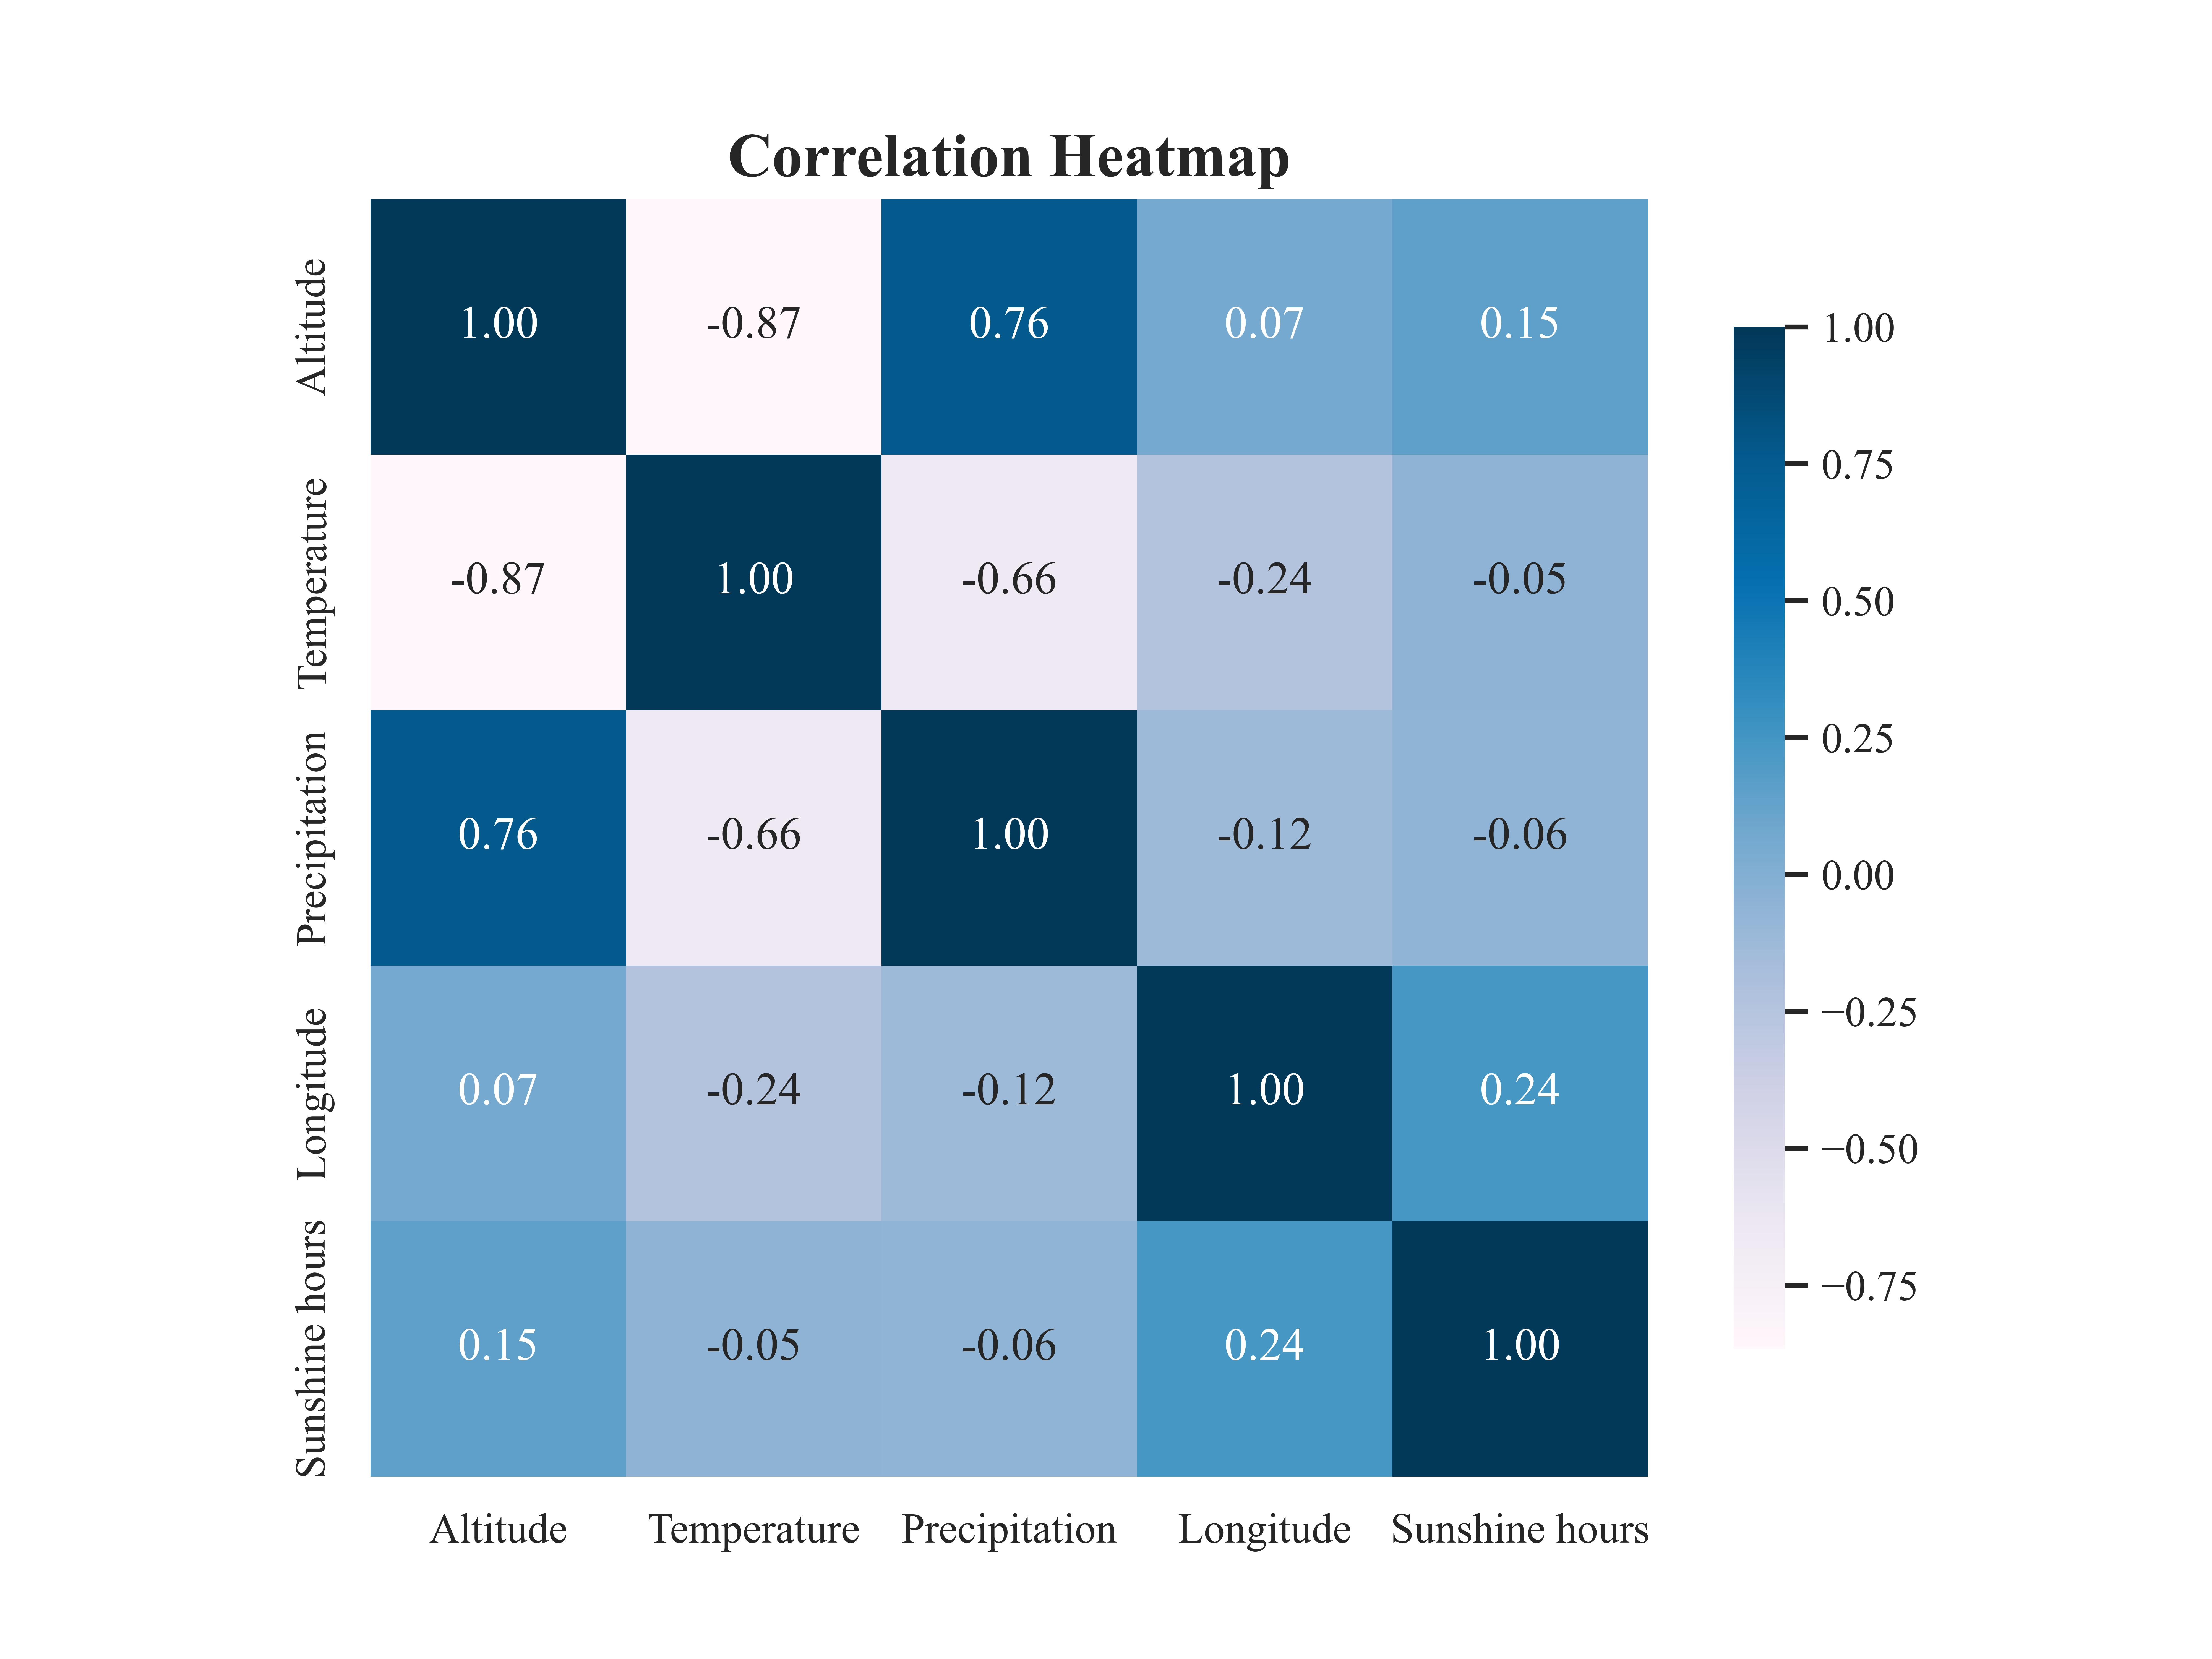
\includegraphics[width=\linewidth]{dataset/DWD/output_graph/eda_corr.jpg}
        \caption{\label{fig:corr}Correlation Heatmap of Variables}
    \end{figure}
\end{minipage}

\section{Discovery Procedure}
In this section, we provide a detailed description of the causal discovery process implemented by Causal Copilot. We also provide the chosen algorithms and hyperparameters, along with the justifications for these selections.

\subsection{Data Preprocessing}
In this initial step, we preprocessed the data and examined its statistical characteristics. This involved cleaning the data, handling missing values, and performing exploratory data analysis to understand distributions and relationships between variables.

\subsection{Algorithm Selection assisted with LLM}
Following data preprocessing, we employed a large language model (LLM) to assist in selecting appropriate algorithms for causal discovery based on the statistical characteristics of the dataset and relevant background knowledge. The top three chosen algorithms, listed in order of suitability, are as follows:   
        
\begin{itemize}
    \item \textbf{PC}:
    \begin{itemize}
        \item \textbf{Description}: The PC algorithm is a constraint-based method that learns the structure of a causal graph from data by testing conditional independencies between variables. It constructs a directed acyclic graph (DAG) representing the causal relationships.
        \item \textbf{Justification}: Given the dataset's large sample size and the absence of missing values, the PC algorithm is efficient for quickly identifying the causal structure in the data while accommodating the non-linear relationships and continuous nature of the variables.
    \end{itemize}

    \item \textbf{GES}:
    \begin{itemize}
        \item \textbf{Description}: Greedy Equivalence Search (GES) is a score-based causal discovery algorithm that identifies the optimal causal structure by navigating the space of equivalence classes of Directed Acyclic Graphs (DAGs).
        \item \textbf{Justification}: GES is well-suited for large datasets and can handle non-Gaussian distributions, which fits the dataset's characteristics. Its ability to efficiently explore complex search spaces makes it a strong candidate for the dataset.
    \end{itemize}

    \item \textbf{NOTEARS}:
    \begin{itemize}
        \item \textbf{Description}: NOTEARS transforms the combinatorial problem of learning Directed Acyclic Graphs (DAGs) into a continuous optimization problem, making it scalable for large datasets.
        \item \textbf{Justification}: NOTEARS is suitable for this dataset, particularly due to its adaptability to high-dimensional data and its capability to handle non-linear relationships, aligning with the observed relationships in the dataset.
    \end{itemize}
\end{itemize}

\subsection{Hyperparameter Values Proposal assisted with LLM}
Once the algorithms were selected, the LLM aided in proposing hyperparameters for the [ALGO] algorithm, which are specified below:

\begin{itemize}
    \item \textbf{alpha}:
    \begin{itemize}
        \item \textbf{Value}: 0.01
        \item \textbf{Explanation}: Given the large sample size of 349, a lower significance level (0.01) is appropriate to reduce the risk of false positives in identifying true causal relationships. This is especially important given that the dataset is not heterogeneous and the relationships may not be linear.
    \end{itemize}
    
    \item \textbf{indep\_test}:
    \begin{itemize}
        \item \textbf{Value}: fisherz
        \item \textbf{Explanation}: Fisher's Z test is suitable here as the data is continuous. While typically it assumes linearity and Gaussian distribution, the PC algorithm can still effectively utilize Fisher's Z in the context of large sample sizes like 349, despite the noted non-linearities.
    \end{itemize}
    
    \item \textbf{uc\_rule}:
    \begin{itemize}
        \item \textbf{Value}: 0
        \item \textbf{Explanation}: Using the default value of 0 is appropriate as it adheres to the standard PC algorithm approach, which is well-suited for the characteristics of this dataset.
    \end{itemize}
    
    \item \textbf{uc\_priority}:
    \begin{itemize}
        \item \textbf{Value}: 2
        \item \textbf{Explanation}: Prioritizing stronger colliders can enhance the robustness of causal inference. A value of 2 offers a balanced approach to resolve conflicts while being aware of potential relationships that may exist among variables.
    \end{itemize}
\end{itemize}

\subsection{Graph Tuning with LLM Suggestion}
In the final step, we performed graph tuning with suggestions provided by the LLM. We utilize LLM to help us determine the direction of undirected edges according to its knowledge repository. By integrating insights from the LLM to refine the causal graph, we can achieve improvements in graph's accuracy and robustness.

\begin{itemize}
    \item \textbf{Altitude $\rightarrow$ Precipitation}: Higher altitude often leads to orographic precipitation, where moist air rises over mountains, cools, and condenses, resulting in increased precipitation.
    
    \item \textbf{Sunshine hours $\rightarrow$ Longitude}: Longitude influences geographical and climatic conditions, which can determine the amount of sunshine hours received at a specific location.
\end{itemize}

This structured approach ensures a comprehensive and methodical analysis of the causal relationships within the dataset.

\section{Results Summary}
\begin{figure}[H]
    \centering
    \begin{subfigure}{0.3\textwidth}
        \centering
        \vspace{-0.5cm}
        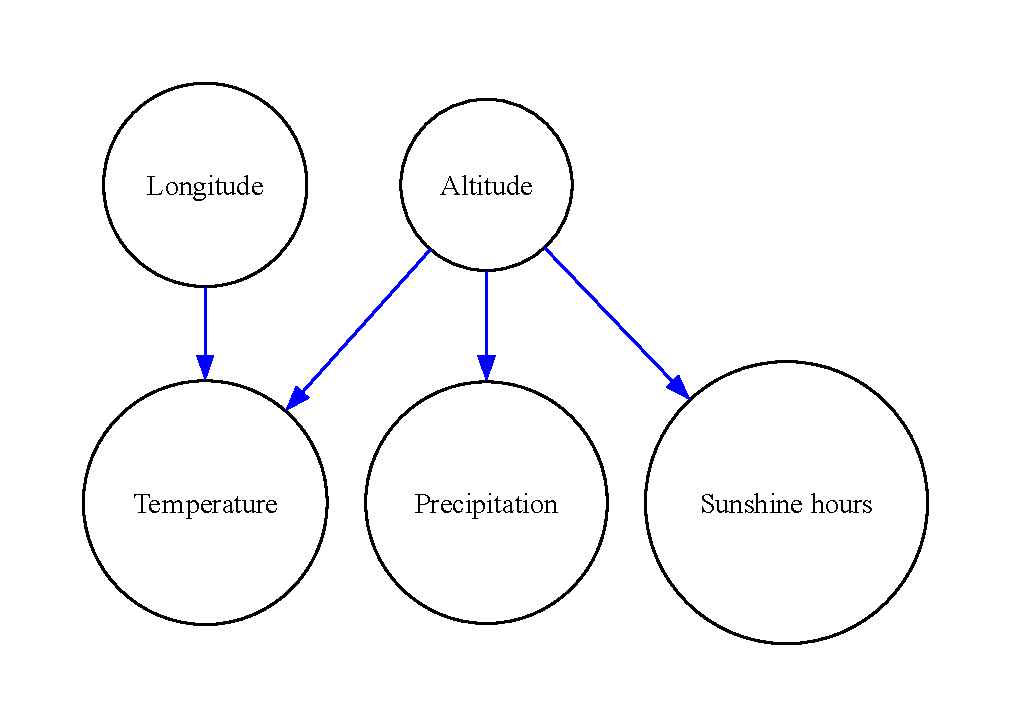
\includegraphics[width=\linewidth]{dataset/DWD/output_graph/true_graph.pdf}
        \vfill
        \caption{True Graph}
        \label{fig:sub1}
    \end{subfigure}
    \hspace{0.04\textwidth}
    \begin{subfigure}{0.3\textwidth}
        \centering
        \vspace{-0.5cm}
        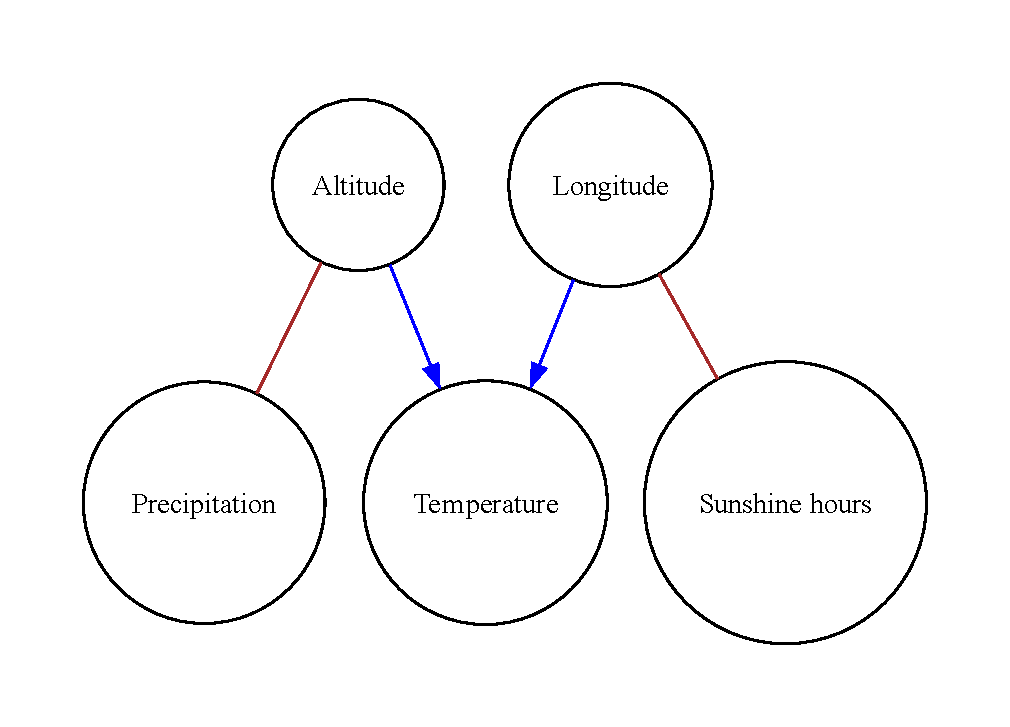
\includegraphics[width=\linewidth]{dataset/DWD/output_graph/initial_graph.pdf}
        \vfill
        \caption{Initial Graph}
        \label{fig:sub2}
    \end{subfigure}
    \hspace{0.04\textwidth}
    \begin{subfigure}{0.3\textwidth}
        \centering
        \vspace{-0.5cm}
        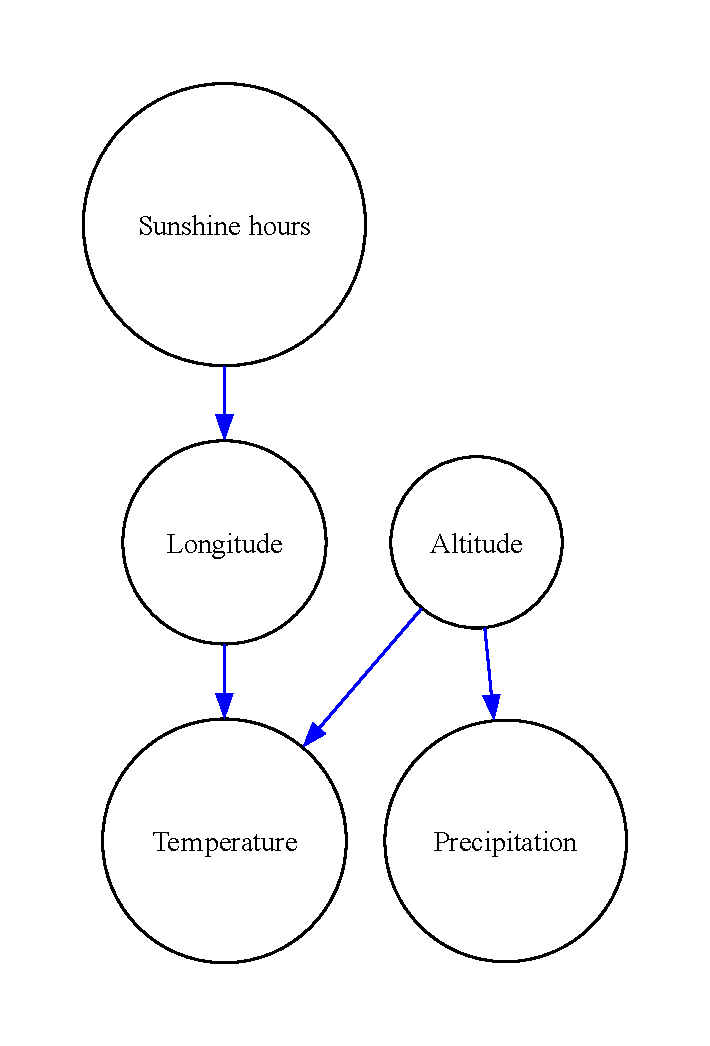
\includegraphics[width=\linewidth]{dataset/DWD/output_graph/revised_graph.pdf}
        \vfill
        \caption{Revised Graph}
        \label{fig:sub3}
    \end{subfigure}
    \caption{Graphs Comparision of PC}
    \label{fig:main}
\end{figure}

The above are result graphs produced by our algorithm. The initial graph is the graph in the first attempt, and the revised graph is the one pruned with LLM suggestion.

The causal relationships among the variables reveal a complex interplay influenced by geographic and atmospheric factors. Altitude impacts Temperature, as higher elevations typically result in lower temperatures due to thinner air and reduced atmospheric pressure. Additionally, altitude also affects Precipitation, as mountains can induce orographic lift, leading to increased rainfall in higher regions. Interestingly, Precipitation appears to have a feedback effect on Altitude, suggesting that the accumulation of precipitation may contribute to geological processes that shape landforms over time. Furthermore, Longitude affects Temperature, likely due to variations in climate zones across different longitudes, which influence average temperatures. Longitude is also linked to Sunshine hours, as geographical position determines the amount of sunlight received throughout the year. There is a reciprocal influence between Sunshine hours and Longitude, indicating that changes in sunlight exposure may also reflect variations in longitudinal positioning. Overall, these connections highlight the dynamic interactions among altitude, temperature, precipitation, longitude, and sunshine hours in shaping climatic and environmental patterns.

\subsection{Graph Reliability Analysis}
\begin{figure}[H]
        \centering
        \vspace{-0.5cm}
        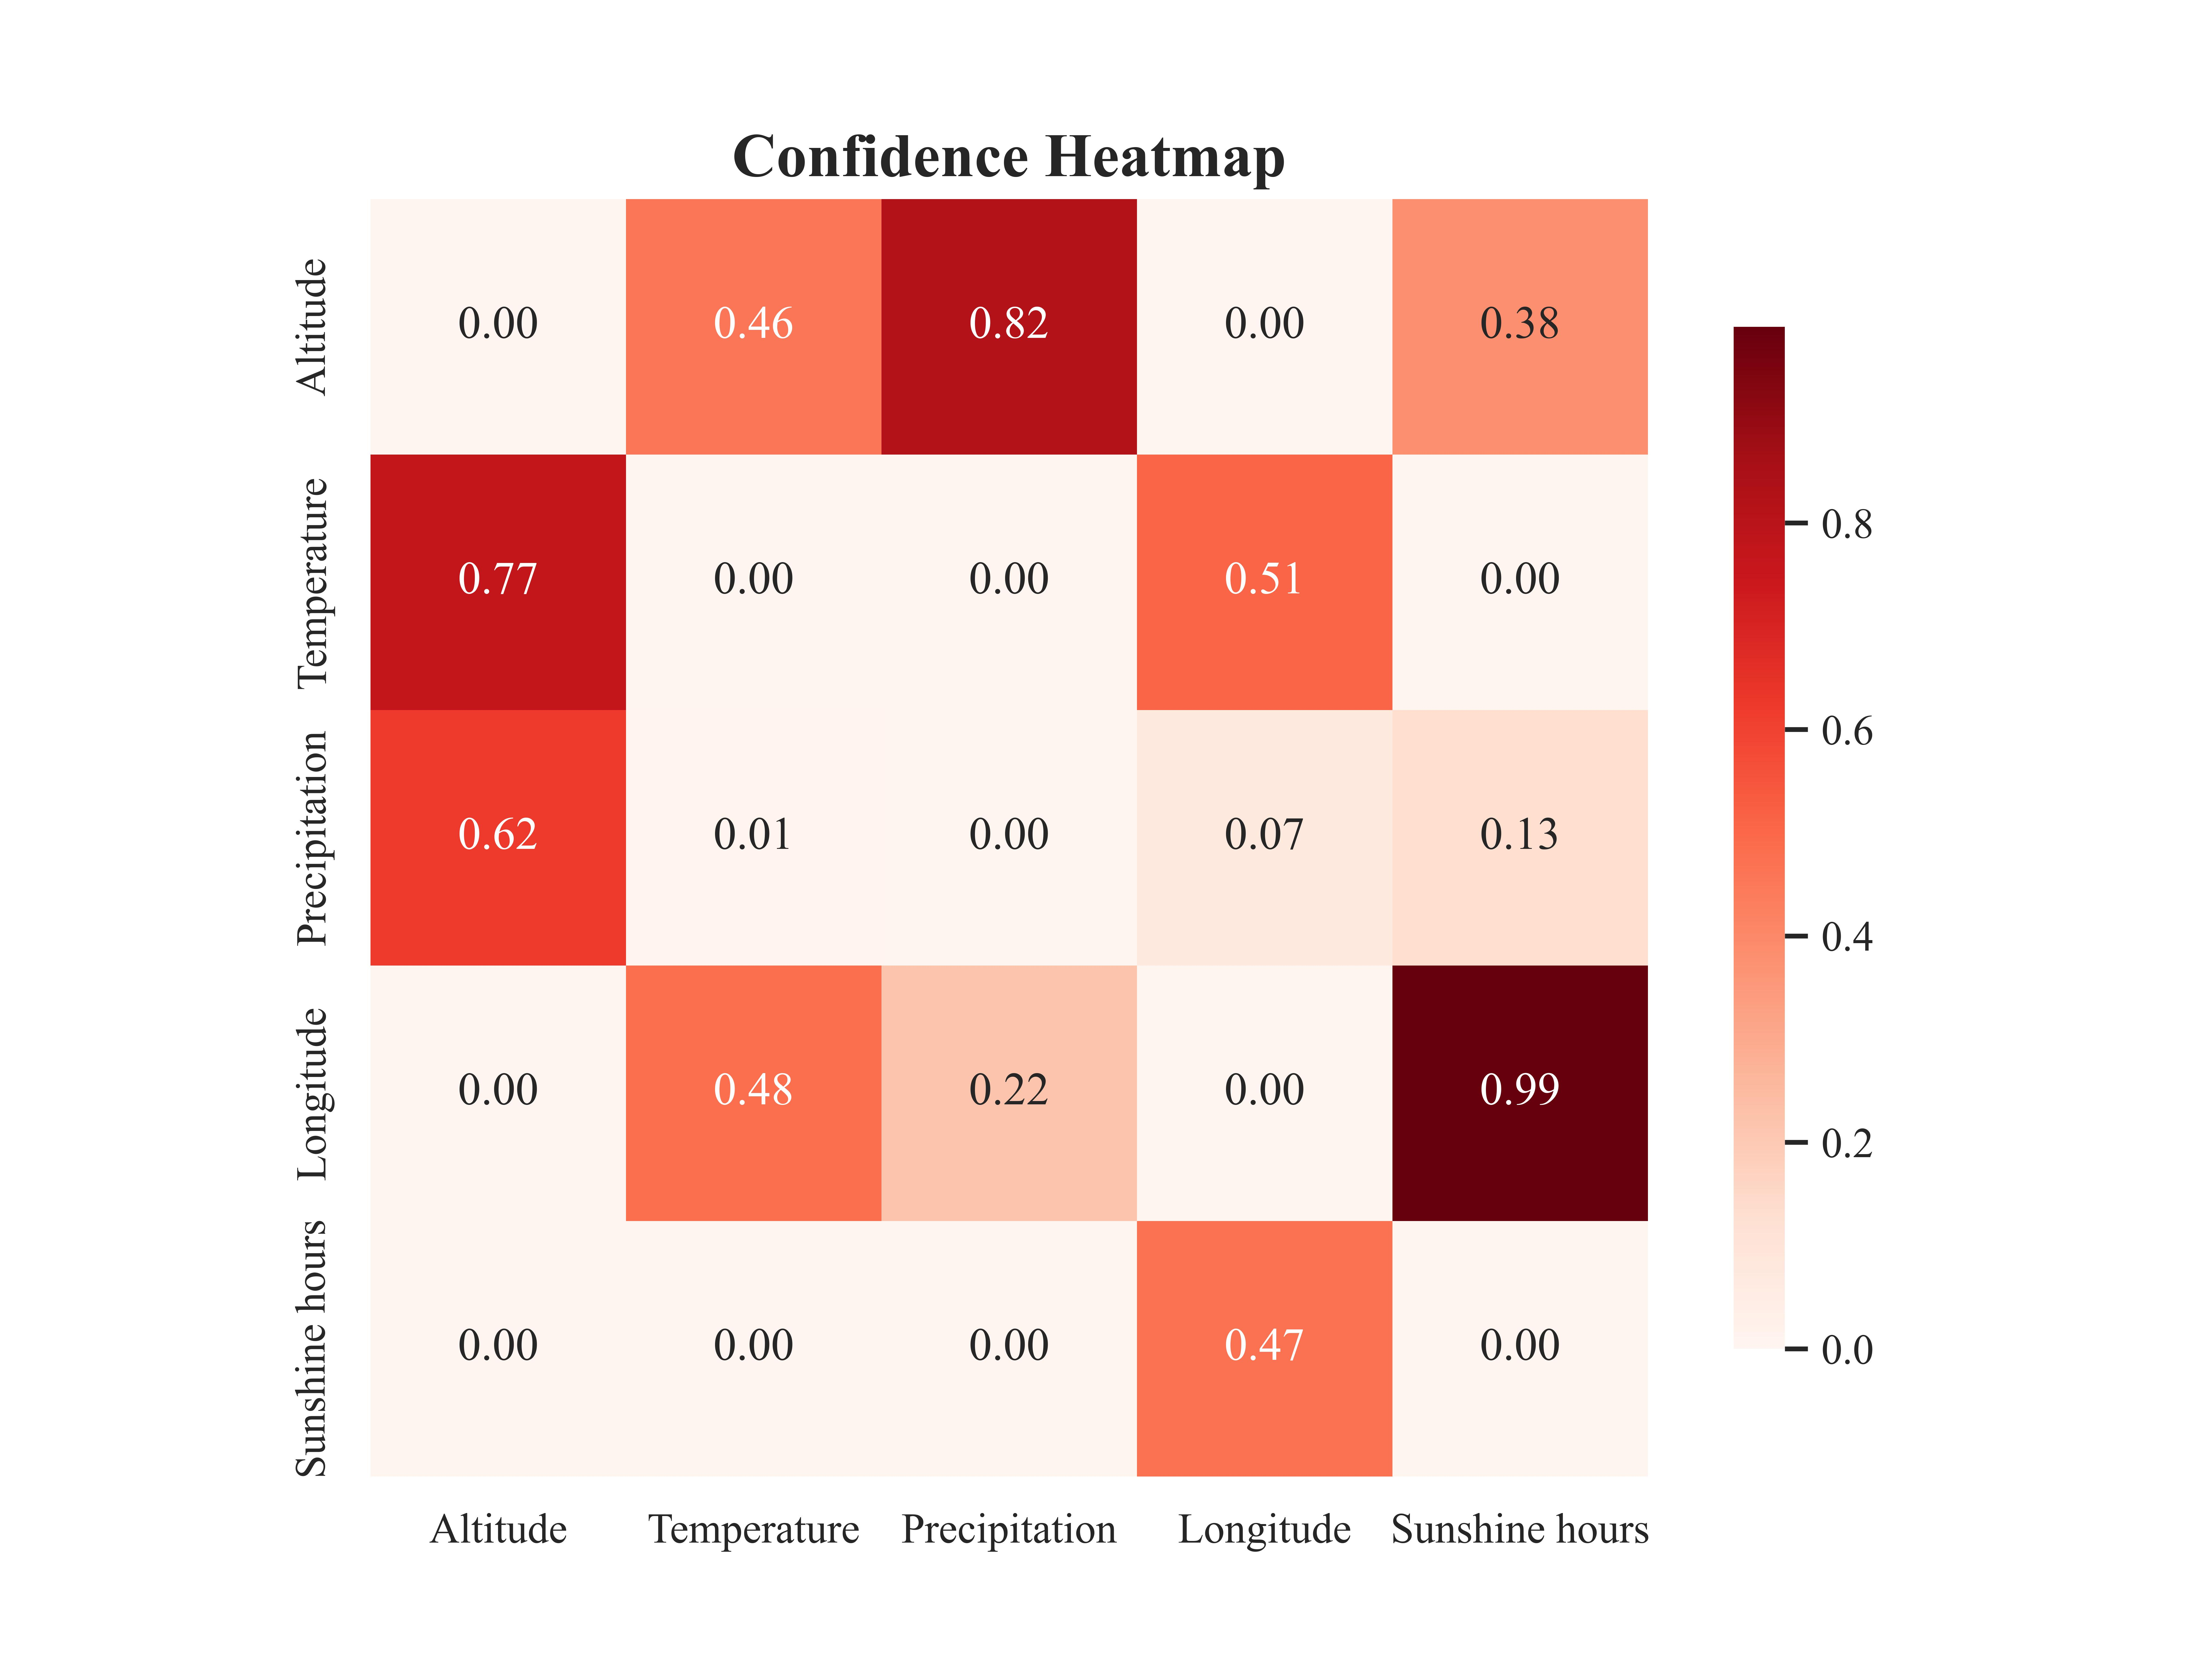
\includegraphics[width=0.8\linewidth]{dataset/DWD/output_graph/confidence_heatmap.jpg}
        \caption{Reliability Graph}
        \label{fig:sub3}
\end{figure}

Based on the confidence probability heatmap and background knowledge, we can analyze the reliability of our graph.

From the statistics perspective, we have high confidence to believe that the edge between Longitude and Sunshine hours exists (bootstrap probability of 0.99), and the edge between Altitude and Temperature exists (bootstrap probability of 0.46) does not hold much confidence. Additionally, we observe that the edges Altitude $\rightarrow$ Precipitation (0.82) and Precipitation $\rightarrow$ Altitude (0.62) show reasonably high bootstrap probabilities, suggesting a strong mutual influence. The edge between Longitude and Temperature (0.48) also lacks sufficient confidence, while the edge Sunshine hours $\rightarrow$ Longitude (0.47) indicates a low likelihood of a causal relationship.

However, based on expert knowledge, we know that it is widely understood that higher altitudes typically result in lower temperatures, supporting the idea that altitude influences temperature despite the low bootstrap probability. Furthermore, orographic precipitation due to altitude reinforces the edge between Altitude and Precipitation. The relationship between Sunshine hours and Precipitation can also be rationalized based on geographical and climatological patterns, where locations with higher sunshine hours typically correlate with lower precipitation, reinforcing the idea of a causal connection.

Therefore, while certain edges, particularly those involving Longitude and Temperature, show low statistical confidence, expert knowledge supports the existence of relationships primarily between Altitude, Temperature, and Precipitation. As such, the result of this causal graph can be considered partially reliable, needing careful interpretation and possibly further analysis to validate uncertainty in less confident edges.

\end{document}